\section{Results}
\subsection{Observed Regression Towards the Median}
In Figure \ref{obs-1}, we plot $m_i-g_i$ (the observed difference) against $g_f-g_i$ (change in grade) for those participants that changed their grades.
\begin{figure*}[h!]
  \centering
    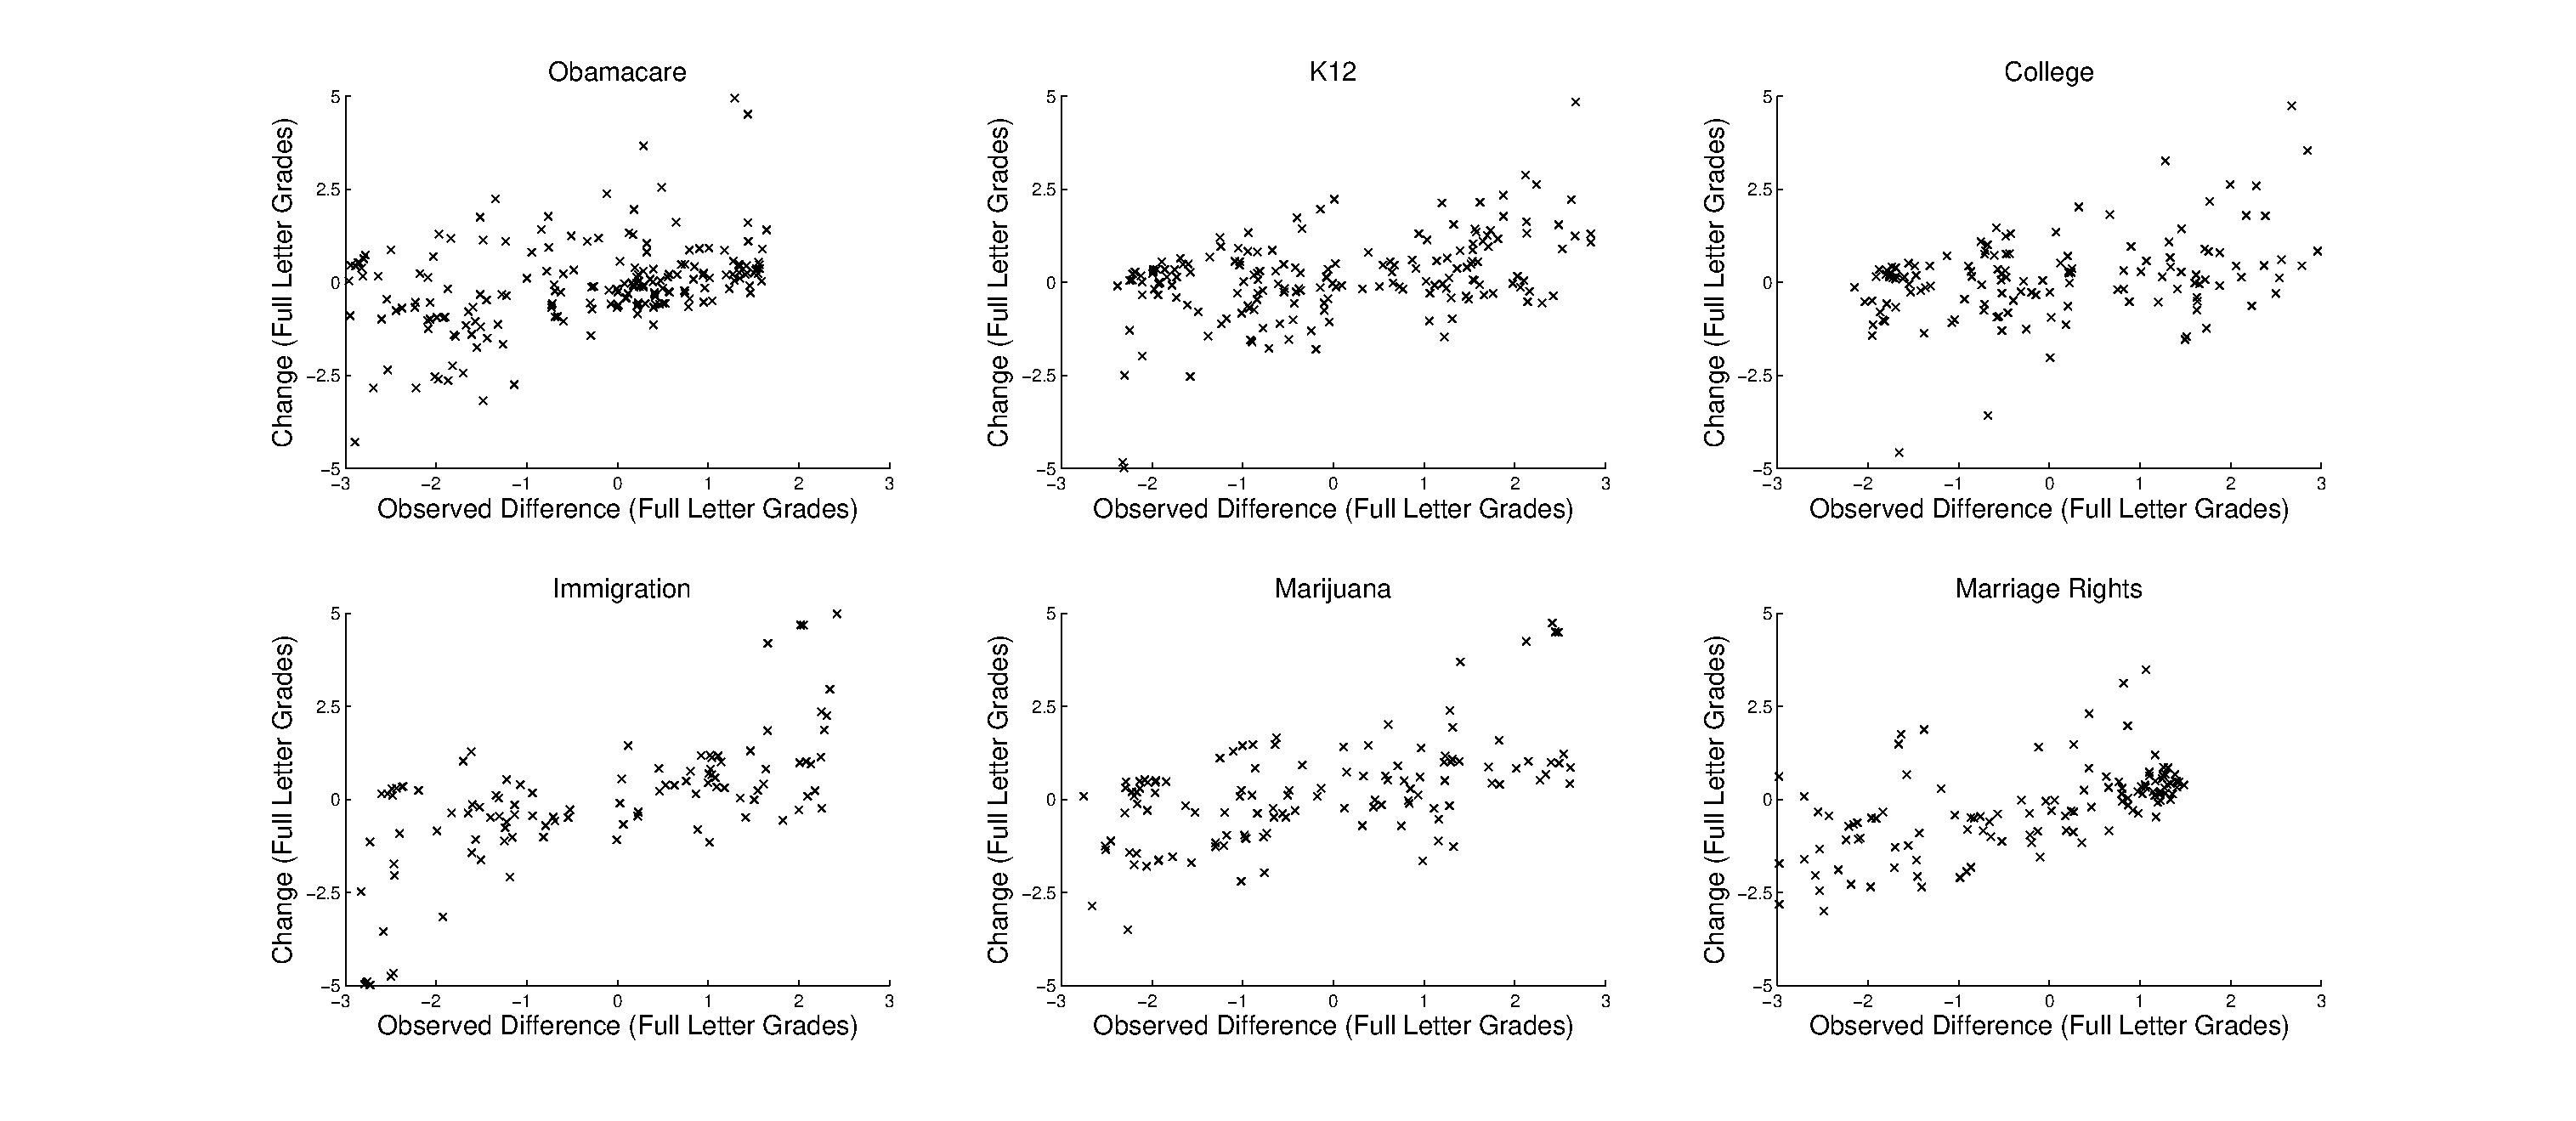
\includegraphics[scale=0.25]{../plots/bias-1.eps}
      \caption{\textbf{TODO}}
      \label{obs-1}
\end{figure*}
Supporting our initial hypothesis, we find that the values are positively correlated, which we define as a change towards the median.

\begin{tabular}[!ht] { r | r | r | r }
  Issue & N &Corr & P-Value \\
  \hline
  \hline
  Obamacare & 223 & 0.4580 & 5.1270e-20 \\
  \hline
  K12 & 172 &0.4813 & 1.6573e-18 \\
  \hline
  College & 139 &0.4263 & 3.9772e-13 \\
  \hline
  Immigration & 105 &0.5856 & 1.8984e-20 \\
  \hline
  Marijuana & 118 &0.5397 & 3.0882e-19 \\
  \hline
  Marriage Rights & 105 & 0.5538 & 4.0921e-25 \\
\end{tabular}

Furthermore, the correlations are significant with respect to the null correlation hypothesis.
The significance test shows it is highly unlikely that there is no correlation between the observed difference and the change in grade.
Note that we discussed that this correlation does not on its own imply a tendency to regress towards the median grade as disccused in Section \ref{ht}, as other models could result in similar correlations.

\subsection{Non-Parametric Test Of Distance From the Median}
We applied the non-parametric test proposed in Section \ref{ht}. 
Figure \ref{dev-1} shows the mean absolute deviation for each group, and Table \ref{dev-2} tests its significance.
\begin{figure}[h!]
  \centering
    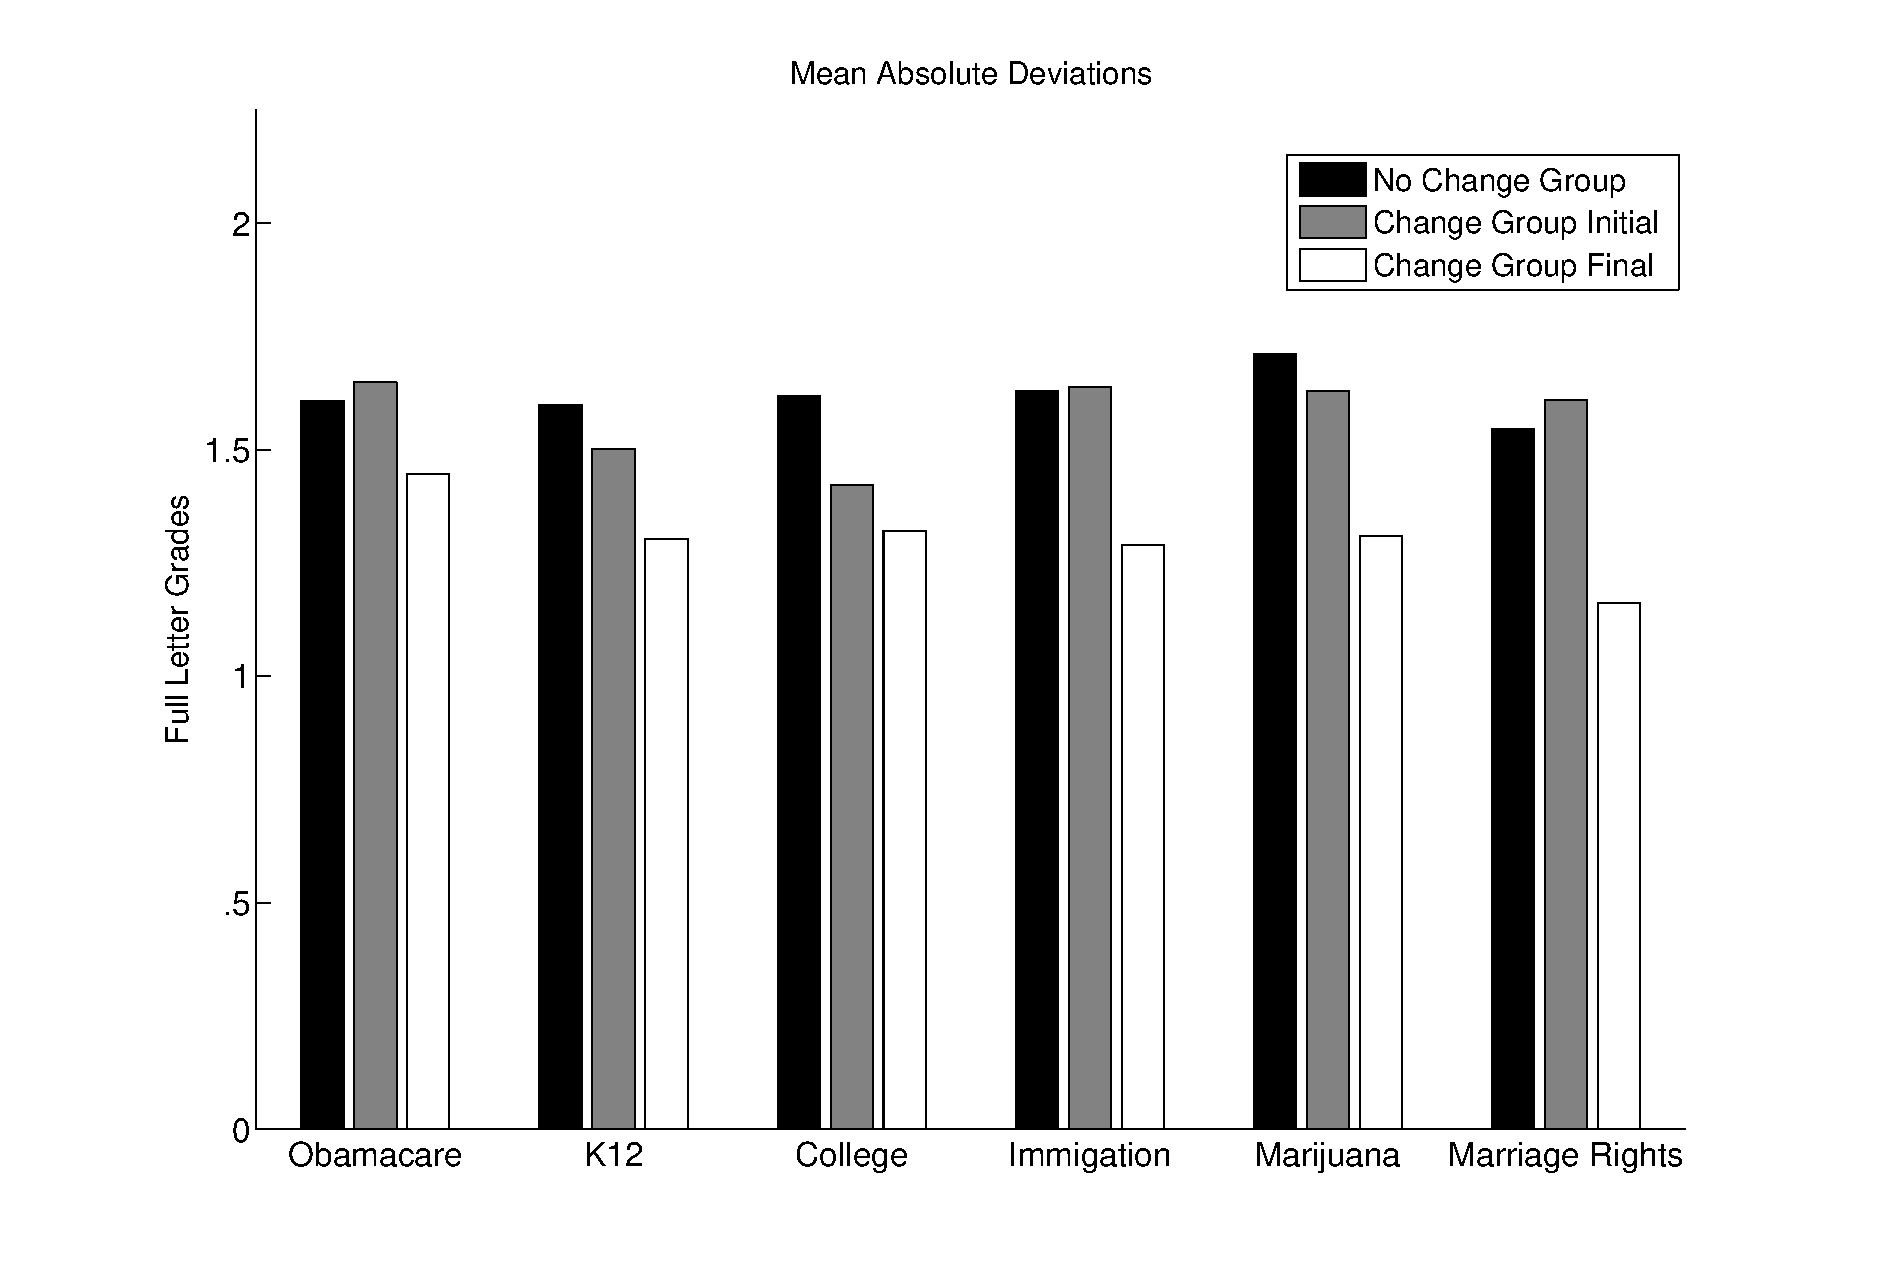
\includegraphics[width=\columnwidth]{../plots/abs-deviations-1.eps}
      \caption{\textbf{TODO}}
      \label{dev-1}
\end{figure}

\begin{tabular}[!ht] { r | r | r }
\label{dev-2}
  Issue & P ($X_c$ vs. $X_n$) & P ($X_c'$ vs. $X_c$)\\
  \hline
  \hline
  Obamacare &  0.0286 & 0.0161 \\
  \hline
  K12 & 2.1314e-06 &  0.0086 \\
  \hline
  College & 1.3033e-04 & 0.0415 \\
  \hline
  Immigration & 7.3456e-07 &4.4170e-05\\
  \hline
  Marijuana & 2.7549e-10 & 4.2560e-05\\
  \hline
  Marriage Rights & 3.5946e-06 & 2.4644e-10 \\
\end{tabular}

For all of the issues, we find that set of absolute deviations from the median $X_c$ is statistically significantly smaller compared to both $X_n$ and $X_c'$.
This suggests that the participants that changed their grades tended to be more tightly centered around median grade.

\subsection{Sequence Dependence}
Using the model proposed in Section \ref{path}, we calculated the test statistics for both the CRC and the Reference Survey.
We found that for all issues the statistic was higher for the CRC suggesting an effect corroborating results in other work such as \cite{???}.
However, none of the results passed a $p < 0.05$ statistical significance test.
\begin{figure}[h!]
  \centering
    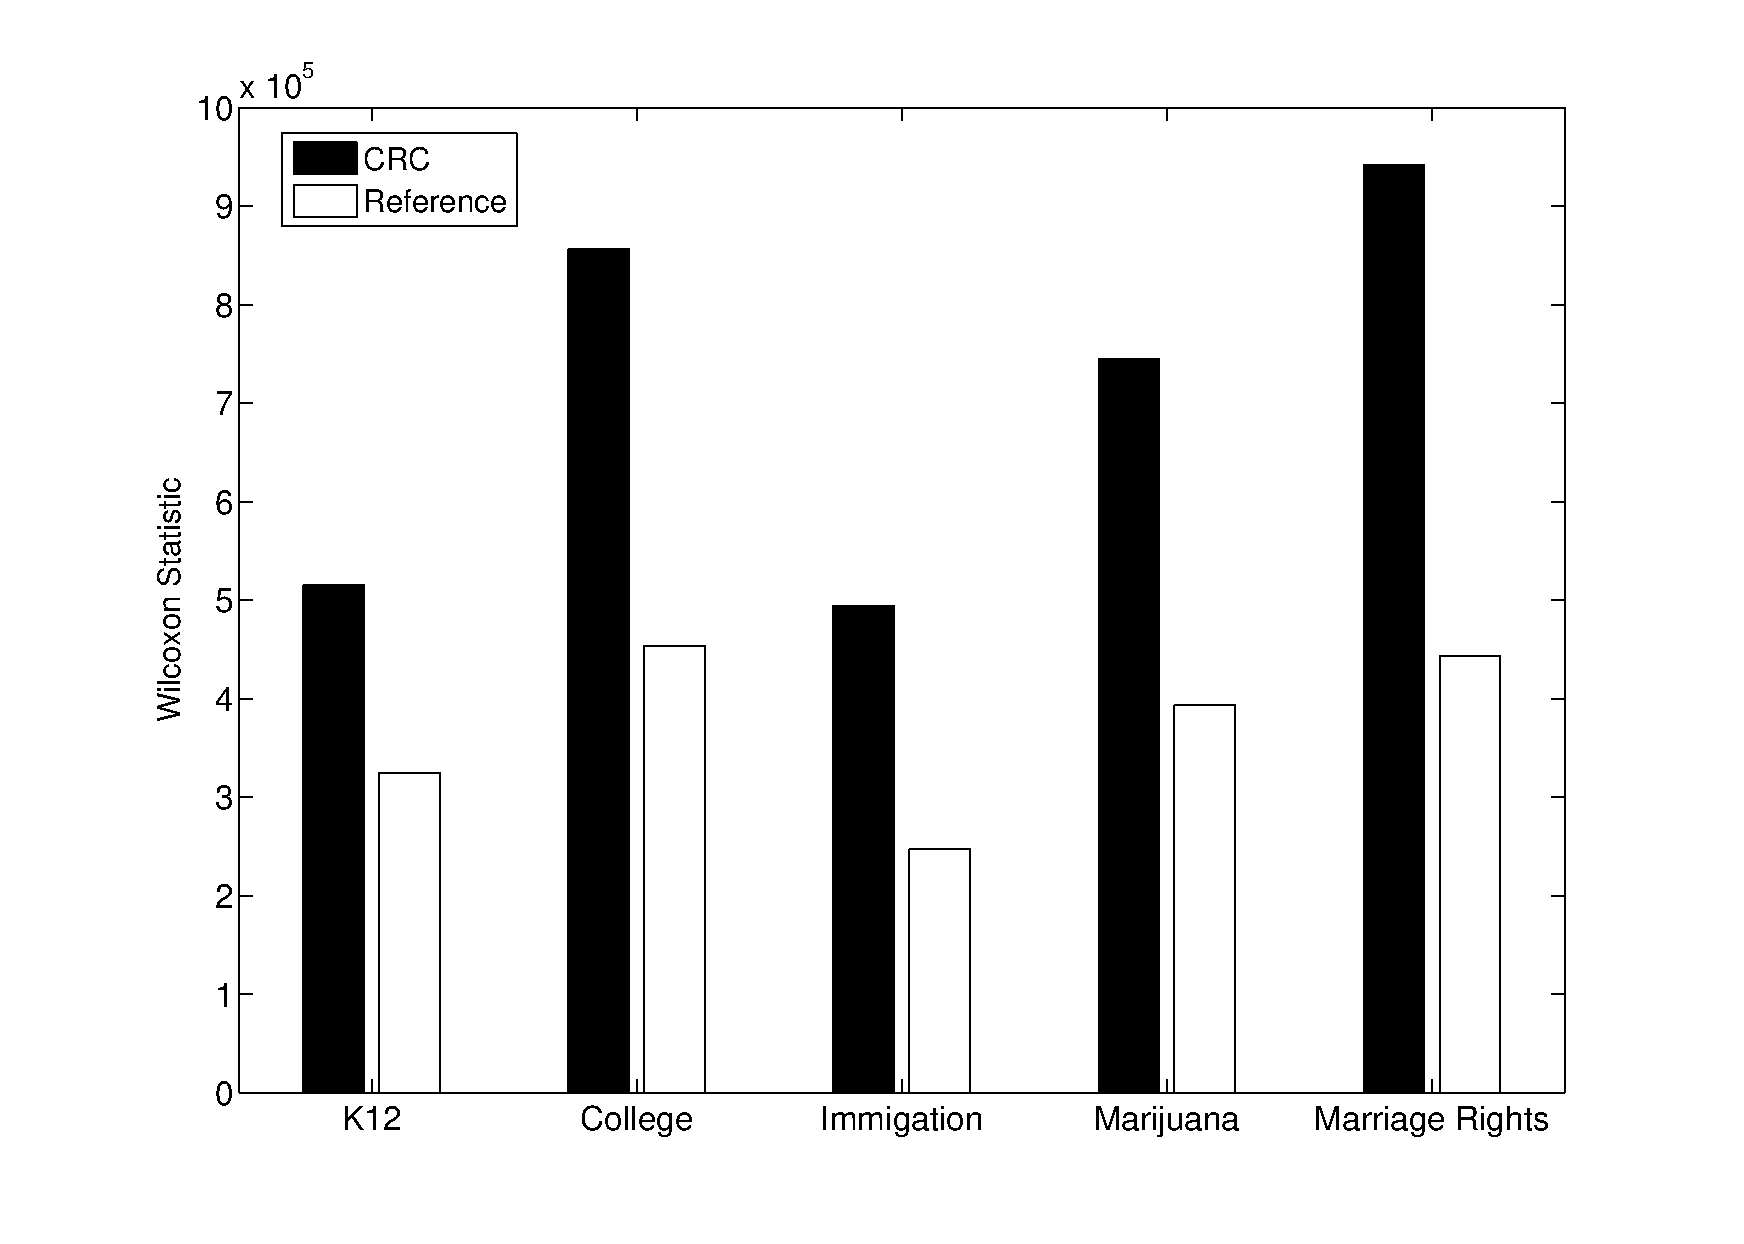
\includegraphics[width=\columnwidth]{../plots/path-dependence.eps}
      \caption{\textbf{TODO}}
      \label{path-1}
\end{figure}
We believe that these results suggest that there is some sequence dependence in the CRC, however, we cannot definitively conclude that from the current quantity of data.

\subsection{Grade Change Model}
In Figure \ref{opt-1} and Figure \ref{opt-2}, we show the results of our model search and locally optimal model for each issue.
We found for four out of the six issues, K12, College, Immigration, and Marijuana, the model we found was linear.
However, for Obamacare and Marriage Rights, we found that the relationship was quadratic.

\begin{figure*}[h!]
  \centering
    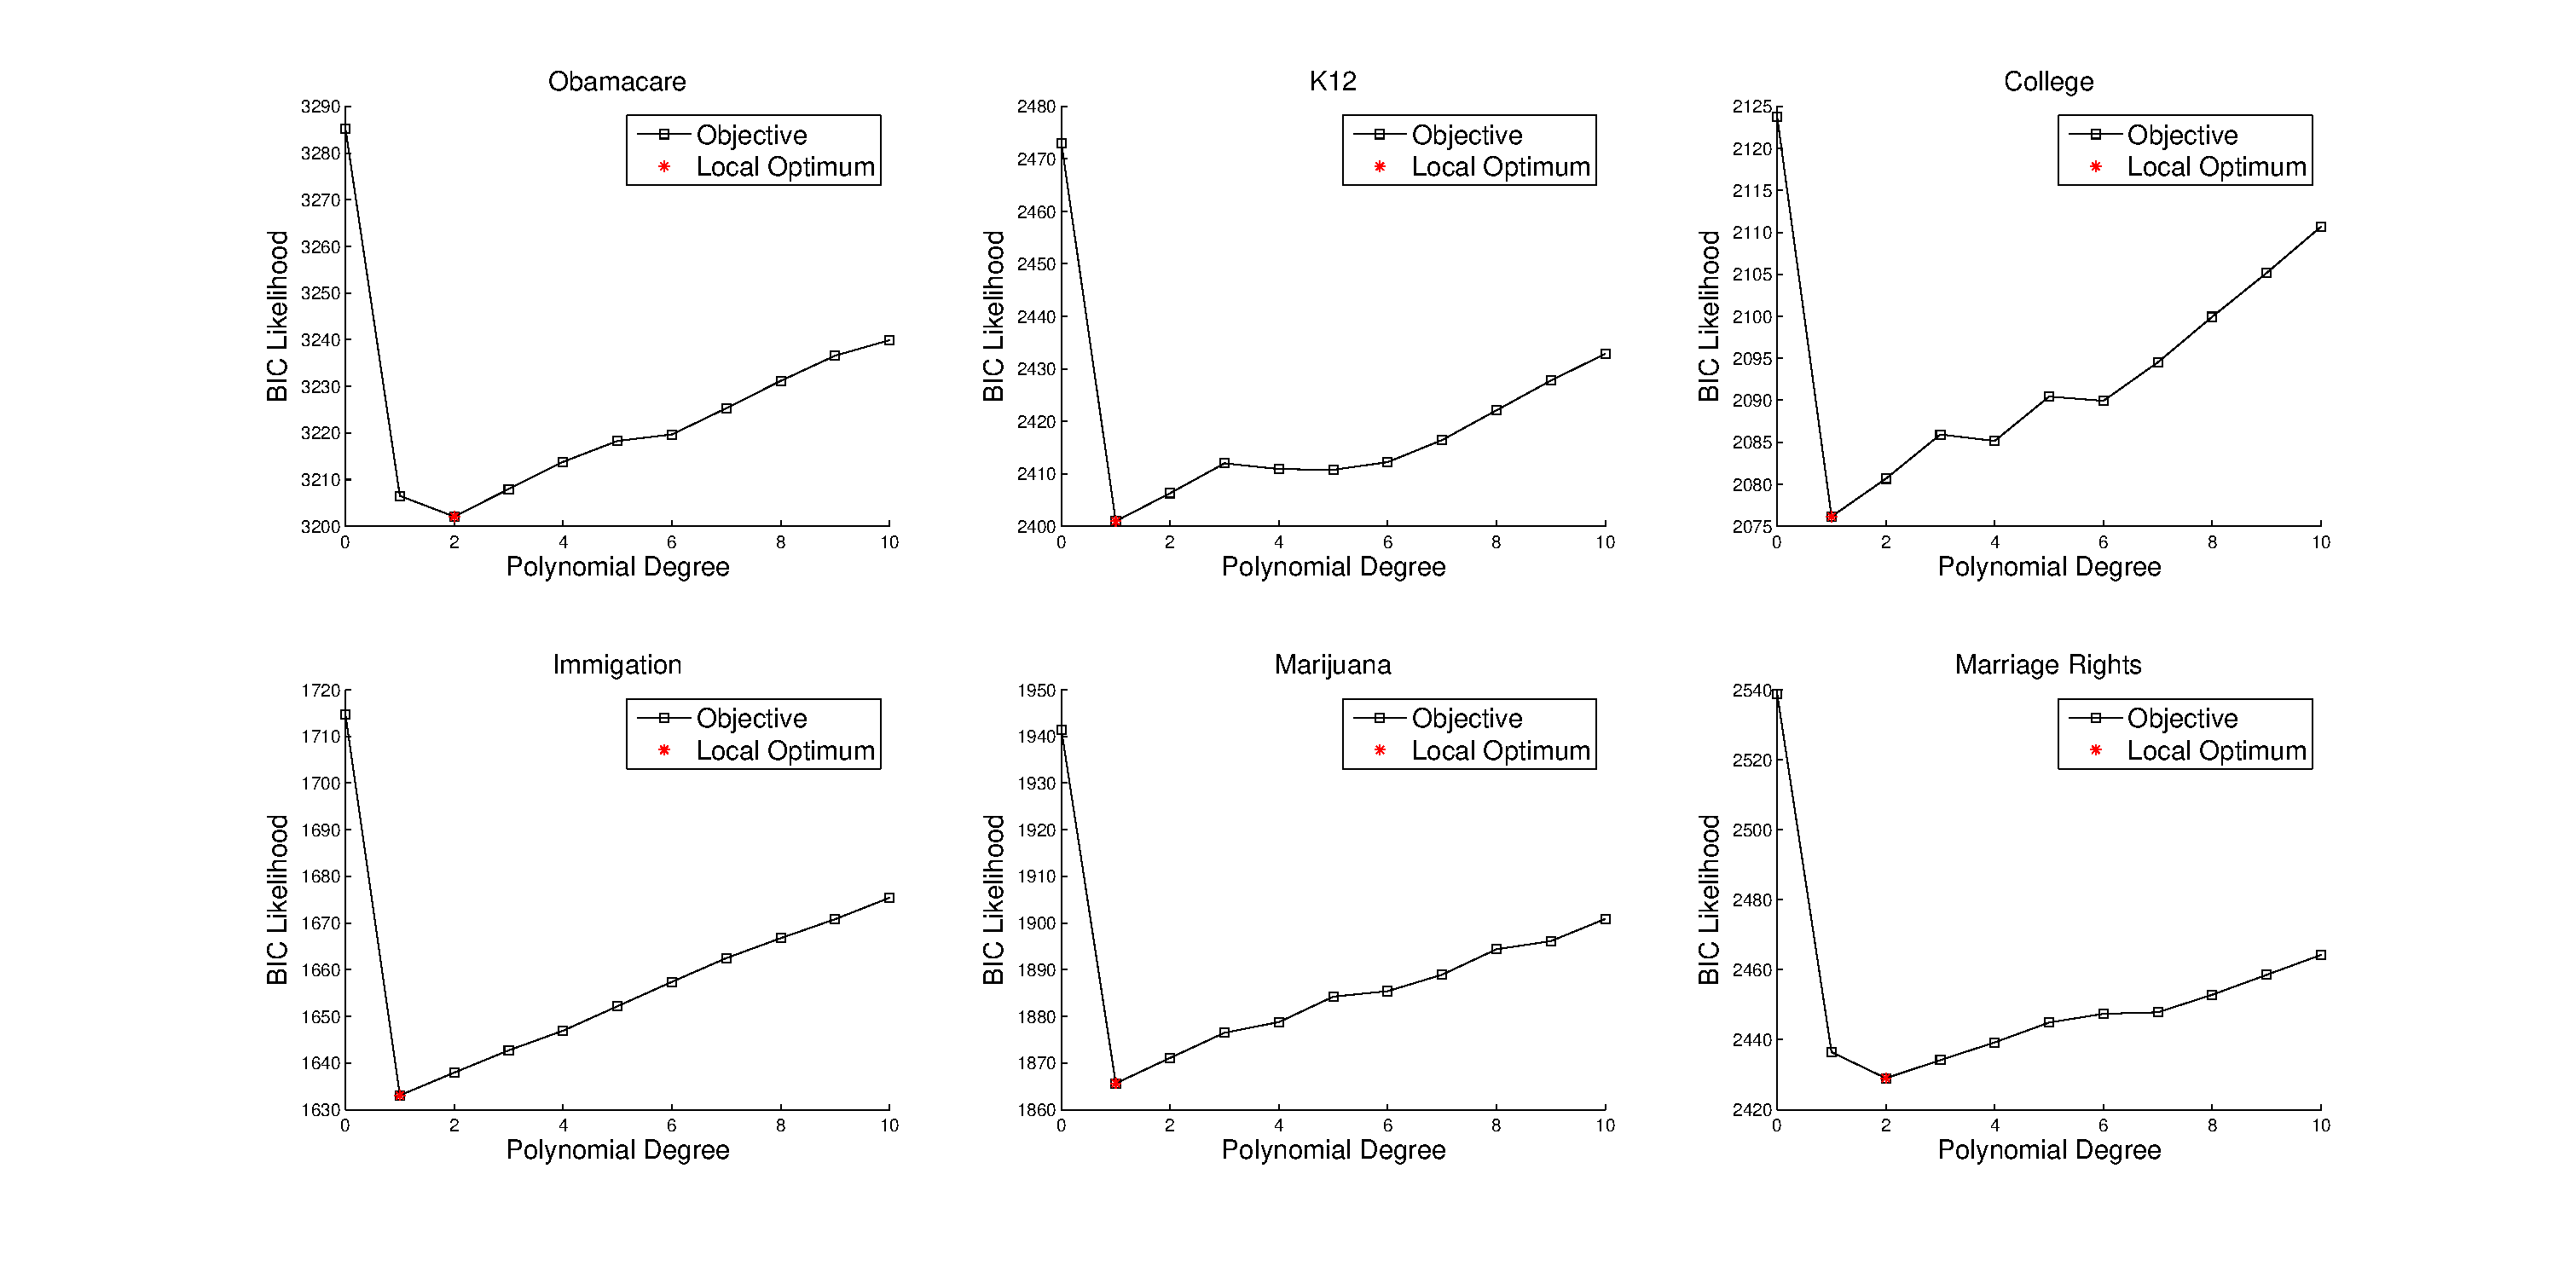
\includegraphics[scale=0.25]{../plots/BIC-optimization.eps}
      \caption{\textbf{TODO}}
      \label{opt-1}
\end{figure*}

\begin{figure*}[h!]
  \centering
    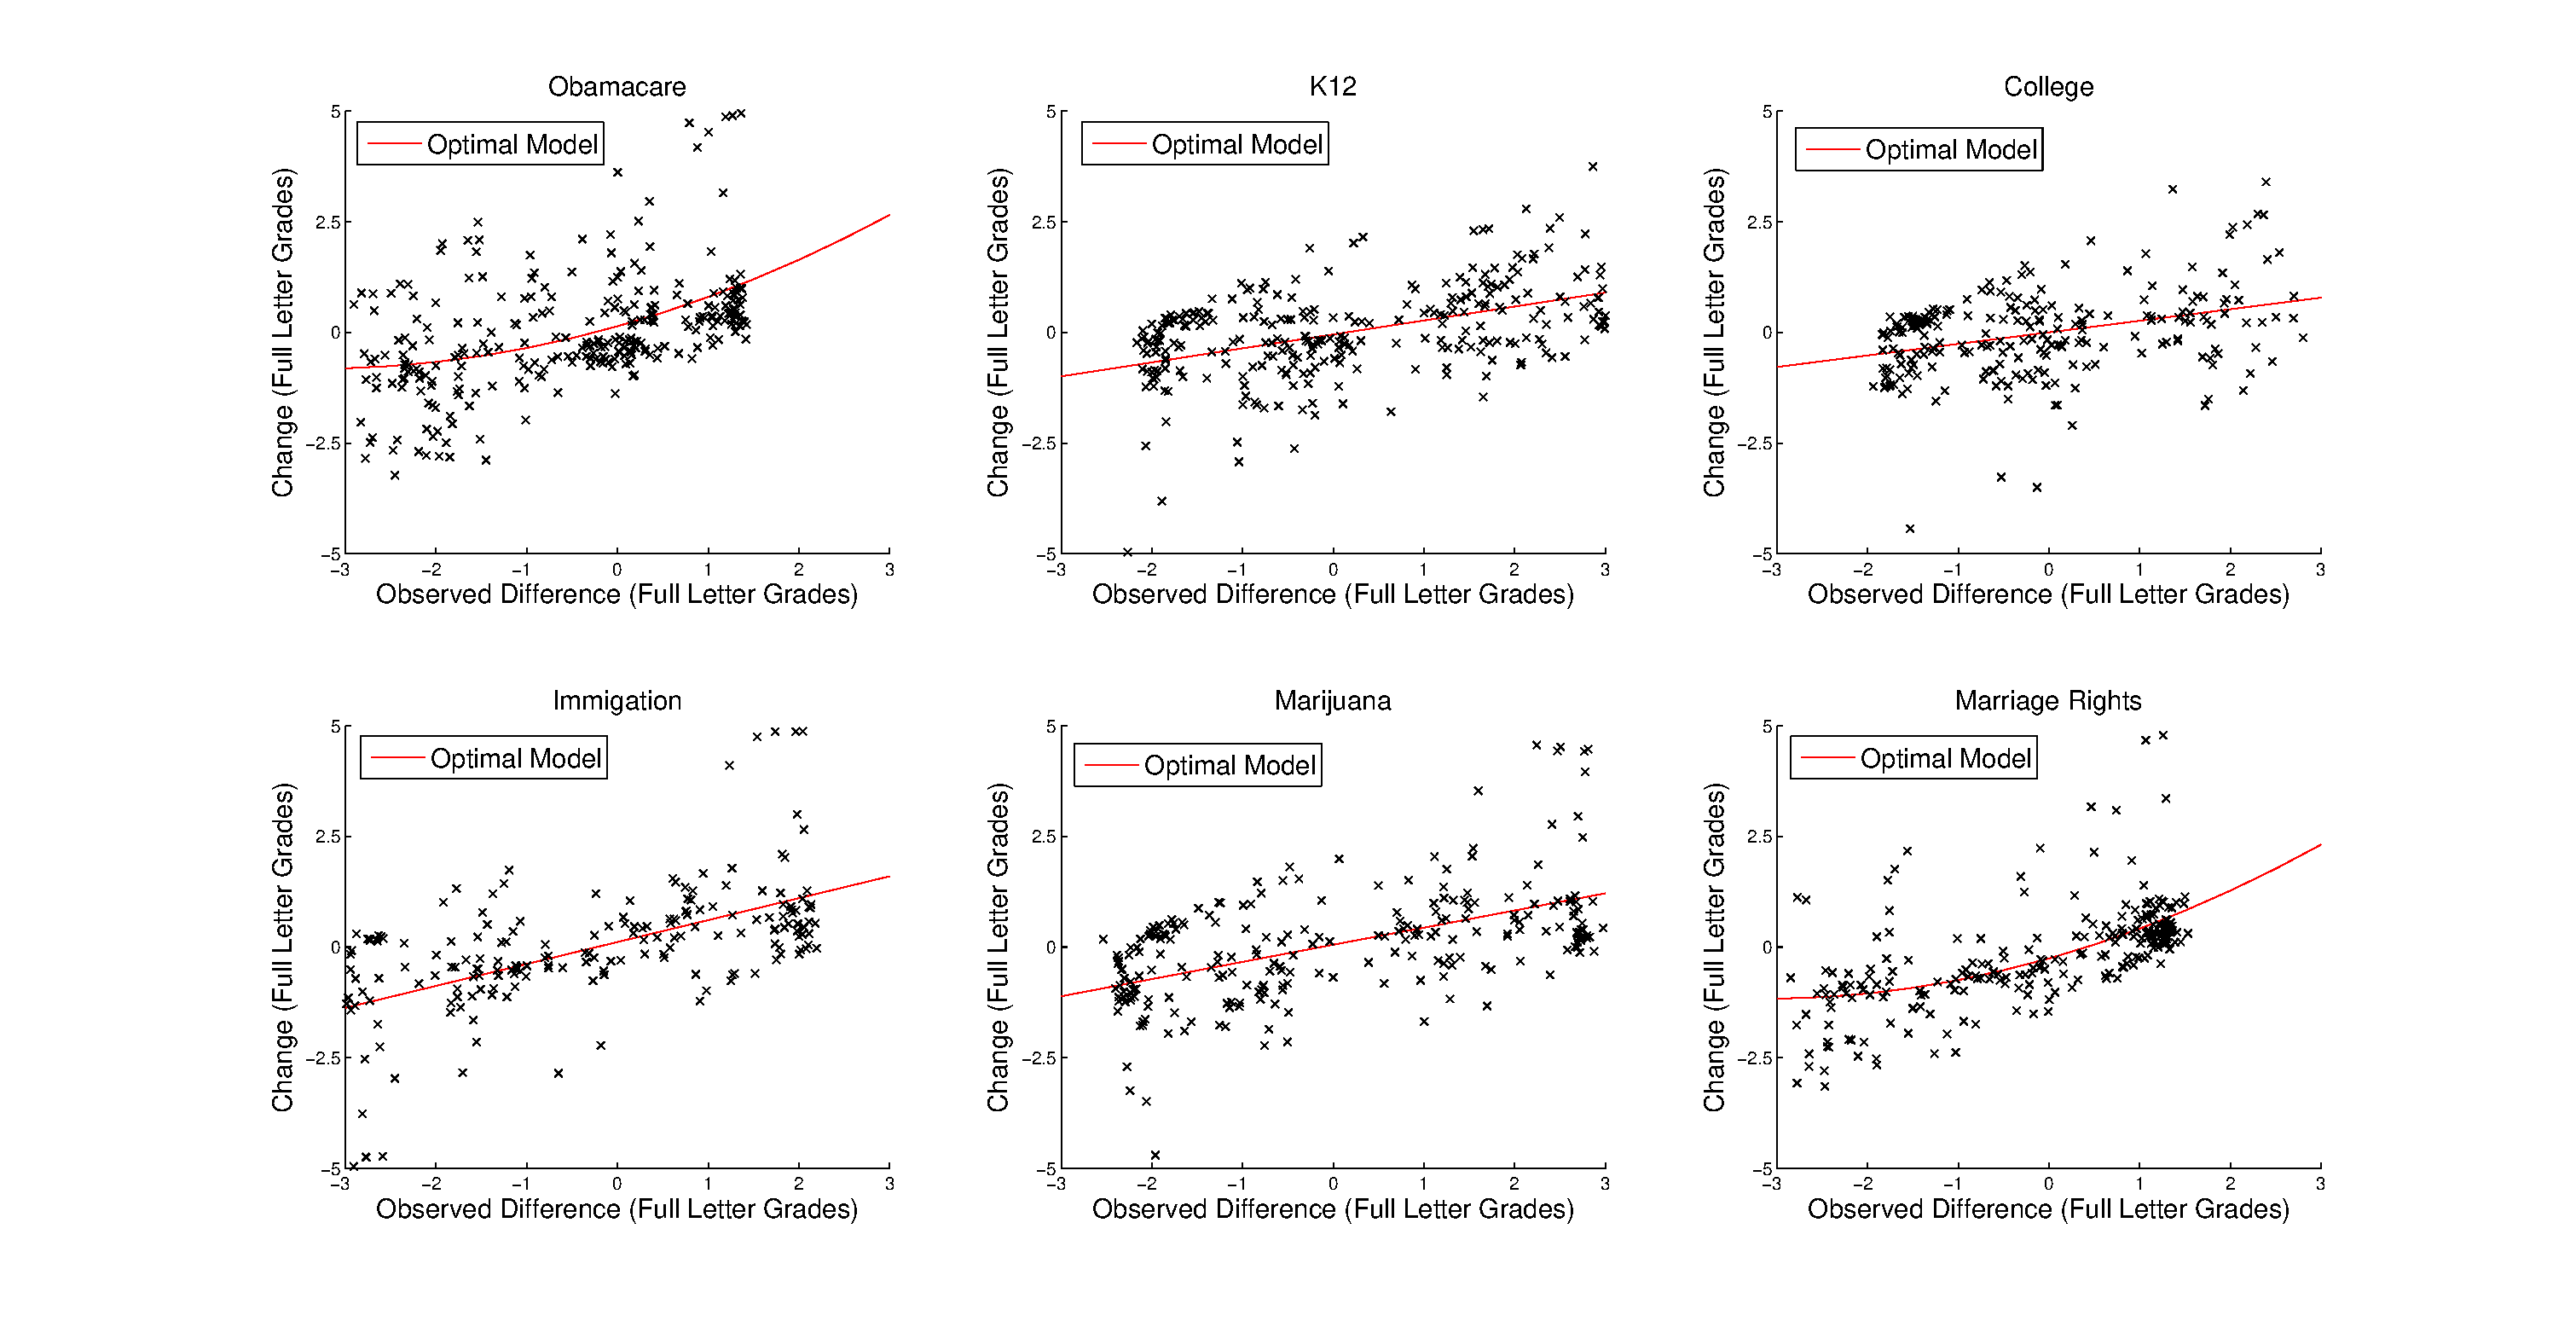
\includegraphics[scale=0.25]{../plots/BIC-optimization-2.eps}
      \caption{\textbf{TODO}}
      \label{opt-2}
\end{figure*}

Figure \ref{opt-2} illustrates the nature of the quadratic relationship, and we see heterogeneity between a positive regression towards the median and a negative regression.
Participants who initially graded the state higher than the median had a more significant tendency to regress downwards.
This result is interesting for a few reasons: (1) contrary to our initial expectations the relationship is largely linear and (2) non-linearities appear in the two issues that received the highest grades which also happen to be highly politicized issues.
There are many possible explanations for this including non-response bias \cite{???} or aversive response \cite{???}; and we defer a more detailed analysis to future work.

\begin{figure}[ht!]
  \centering
    \includegraphics[width=\columnwidth]{../plots/shift-parameter.eps}
      \caption{\textbf{TODO}}
      \label{dev-1}
\end{figure}

\subsection{Shift-parameter estimation}
In Figure \ref{dev-1}, we show the results for the $\Delta$ parameter estimate from inverting our hypothesis test.
We find that on average grades in our change group were about half a letter grade (ie. +, -) closer to the median than grades from participants who didn't change.
This parameter is relevant to both recommender systems and prediction tools.
In the simplest case, if we were to build a grade prediction tool that simply predicted the median grade, we could get misleadingly low prediction error.  
Likewise, algorithms that rely on proximity such as clustering or k-nearest neighbors could be misled to create a single big cluster around the median, when in fact the clustering around the median may be due to a biasing tendency.

\subsection{Comparision To Reference Survey}
We applied our proposed non-parametric test to compare the absolute deviations in the group of participants who changed their grades in the CRC with results from a reference survey.
For the reference survey, we calculated the absolute deviation around the median (which the participants were not shown).
We found for all but one issue the grades from the CRC were statistically significantly closer to the median than ones from the reference survey.

\begin{tabular}[!ht] { r | l | l | r}
\label{ref-1}
  Issue & Med(Ref) & Med(CRC) & p-val \\
  \hline
  \hline
  Obamacare &  B & B & 0.0078\\
  \hline
  K12 & C+ & C & 0.3563\\
  \hline
  College & C- & C- & 0.0011\\
  \hline
  Immigration & C & C+ & 0.0277\\
  \hline
  Marijuana & C & C & 0.0076\\
  \hline
  Marriage Rights & B+ & B+ & 0.0494 \\
\end{tabular}

Furthermore, the two surveys aligned nearly perfectly in aggregate.
